%\vspace{-1mm}
We evaluate our algorithm on three case studies: (1) grid-world, (2) cart-pole, and (3) mountain-car. The cart-pole environment\footnote{\url{https://github.com/openai/gym/wiki/CartPole-v0}} and the mountain-car environment\footnote{\url{https://github.com/openai/gym/wiki/MountainCar-v0}} are obtained from OpenAI Gym. All experiments are carried out on a quad-core i7-7700K processor running at 3.6 GHz with 16 GB of memory. 
Our prototype tool was implemented in Python\footnote{\url{https://github.com/zwc662/CAV2018}}.
For the OpenAI-gym experiments, in each step, the agent sends an action to the OpenAI environment and the environment returns an observation and reward. 
The parameters are $\gamma=0.99, \sigma=10^{-5}, \alpha=0.5$. For grid-world, $\epsilon=1E-5$, whereas for OpenAI-gym environments, $\epsilon=10$.
We use model checking results to show that our algorithm can guarantee the safety of the learnt policy. Moreover, we quantitatively show that the learnt policy has comparable performance compared with the one directly learnt using AL.
%\vspace{-2mm}
\section{Navigation in Grid World}
Our first experiment is an extension on the 2D navigation task in Section~\ref{sec:section3}. Specifications with different $p^*$'s in \label{eq:spec} are given. Fig.~{\ref{fig:grid_world2} shows the different reward mappings that induce the policies learnt by our algorithm. As the safety threshold (value of $p^*$) decreases, the algorithm will try to find a weight vector that assigns low rewards to the  unsafe states and states around them, so that the agent will have a lower probability of moving into the unsafe areas. However, as a result, the agent will also focus more on avoiding the unsafe areas than actually reaching the goal area. In essence, we trade off performance with safety. 
%\vspace{-10mm}
\begin{figure}[!htb]
\centering
\subfigure[]{
	\begin{minipage}[c][0.8\width]{
	   0.3\textwidth}
	   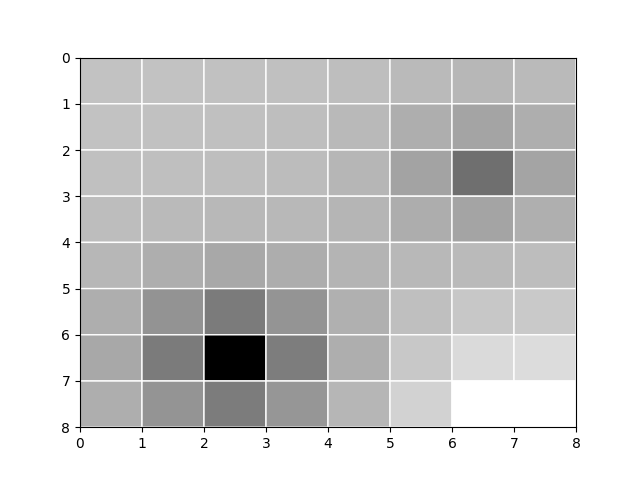
\includegraphics[width=1.\linewidth]{0_9.png}
	   \label{fig:grid_world2a}
	\end{minipage}\hfill
}
%\subfigure[]{
%	\begin{minipage}[c][0.85\width]{
%	   0.2\textwidth}
%	   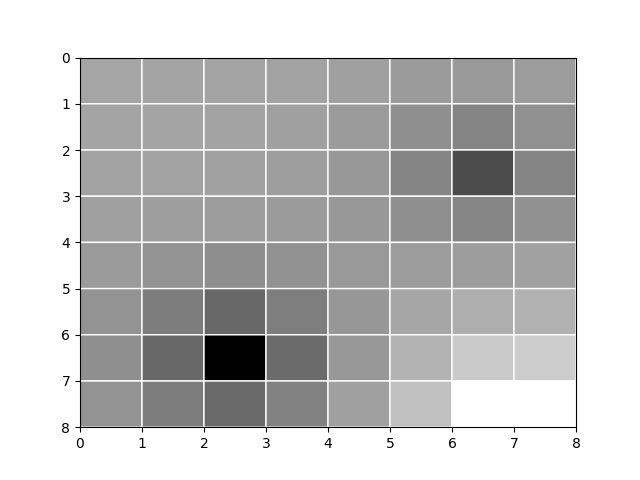
\includegraphics[width=1.2\linewidth]{0_8.png}
%	   \label{fig:grid_world2b}
%	\end{minipage}\hfill
%}
%\subfigure[]{
%	\begin{minipage}[c][0.85\width]{
%	   0.2\textwidth}
%	   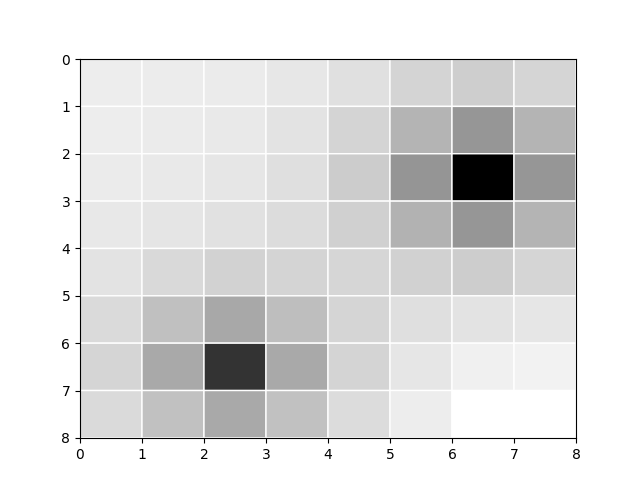
\includegraphics[width=1.2\linewidth]{0_6.png}
%	   \label{fig:grid_world2c}
%	\end{minipage}\hfill
%}
\subfigure[]{
	\begin{minipage}[c][0.8\width]{
	   0.3\textwidth}
	   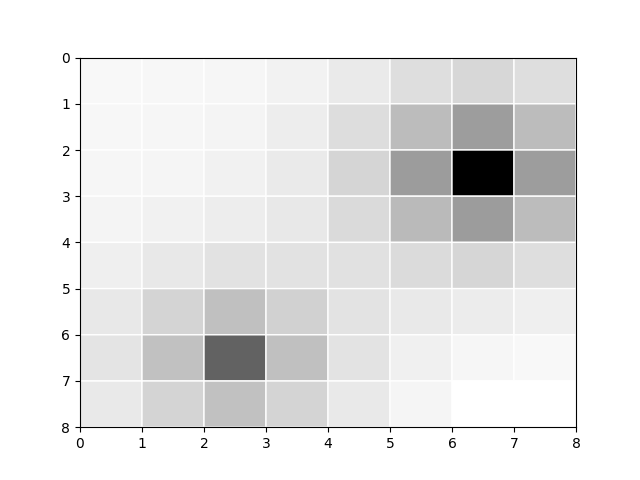
\includegraphics[width=1.\linewidth]{0_4.png}
	   \label{fig:grid_world2d}
	\end{minipage}\hfill
}
%\subfigure[]{
%	\begin{minipage}[c][0.85\width]{
%	   0.2\textwidth}
%	   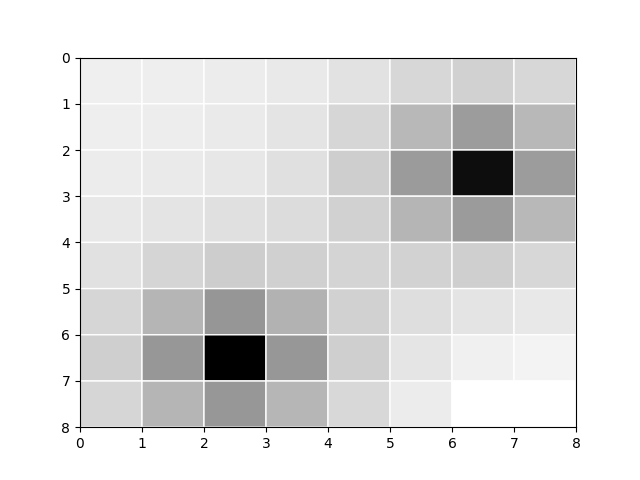
\includegraphics[width=1.2\linewidth]{0_2.png}
%	   \label{fig:grid_world2e}
%	\end{minipage}\hfill
%}
\subfigure[]{
	\begin{minipage}[c][0.8\width]{
	   0.3\textwidth}
	   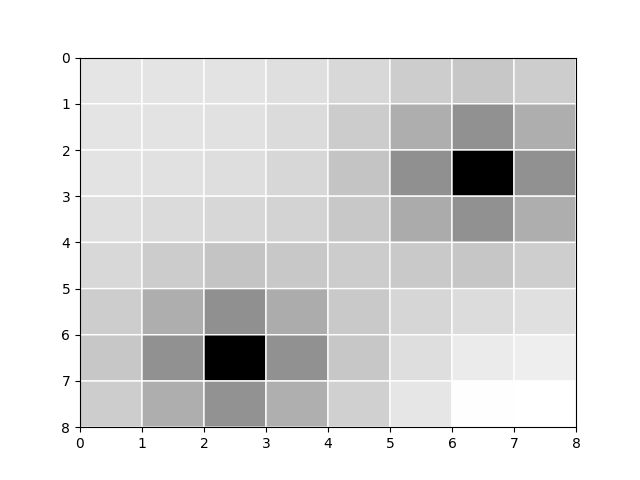
\includegraphics[width=1.\linewidth]{0_1.png}
	   \label{fig:grid_world2f}
	\end{minipage}\hspace{0.012\linewidth}
}
\caption[Reward mappings of gridworld for different safety threshold]
{(a)$p^* = 90\%$. The learnt policy has a probability of $12.5\%$ with respect to the given PCTL property. The reward function assigns lower rewards to the unsafe states than the states nearby. (b) $p^* = 40\%$. The learnt policy has a probability of $11.0\%$ with respect to the given PCTL property. The reward function assigns even lower rewards to the unsafe states, indicated by the greater contrast between unsafe states and other states. (c)$p^* = 10\%$. The learnt policy has a probability of $4\%$ with respect to the given PCTL property. The reward function assigns such low rewards to the unsafe states that the states nearby are also assigned with low rewards (because of the radial basis feature functions).}
\label{fig:grid_world2}
%\vspace{-4mm}
\end{figure}
%\vspace{-6mm}
\begin{table}[htb]
\begin{center}
\caption{Average runtime per iteration in seconds.}
\begin{tabular}{|c|r|r|r|r|r|}
\hline
Size & Num. of States & Compute $\pi$ & Compute $\mu$ & MC & Cex\\
\hline
$8 \times 8$ & 64 & 0.02 & 0.02 & 1.39 & 0.014\\
$16 \times 16$ & 256 & 0.05 & 0.05 & 1.43  & 0.014\\
$32 \times 32$ & 1024 & 0.07 & 0.08 & 3.12 & 0.035\\
$64 \times 64$ & 4096 & 6.52 & 25.88 &  22.877  & 1.59\\
\hline
\end{tabular}
\label{tab:grid-world}
\end{center}
\end{table}
%\vspace{-10mm}
We also evaluated the scalability of our implementation using the grid-world example. The first and second columns indicate the size of the grid world and the resulting state space. The third column shows the average runtime that policy iteration takes to compute an optimal policy $\pi$ for a known reward function. The forth column indicates the average runtime that policy iteration takes to compute the expected features $\mu$ for a known policy. The fifth column indicates the average runtime of verifying the PCTL formula using PRISM. The last column indicates the average runtime that generating a counterexample using COMICS.  


\section{Cart-Pole from OpenAI Gym}
%%\vspace{-8mm}
\begin{figure}[hbt]
  \centering
   	\subfigure[]{
	\begin{minipage}[c][0.35\textwidth]{
	   0.45\textwidth}
	   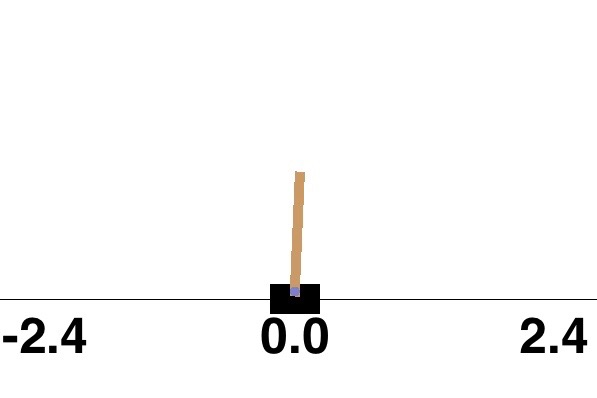
\includegraphics[width=\linewidth]{cartpole-v0.jpg}
	   \label{fig:cartpole-v0}
	\end{minipage}\hfill
}
\subfigure[]{
	\begin{minipage}[c][0.35\textwidth]{
	   0.45\textwidth}
	   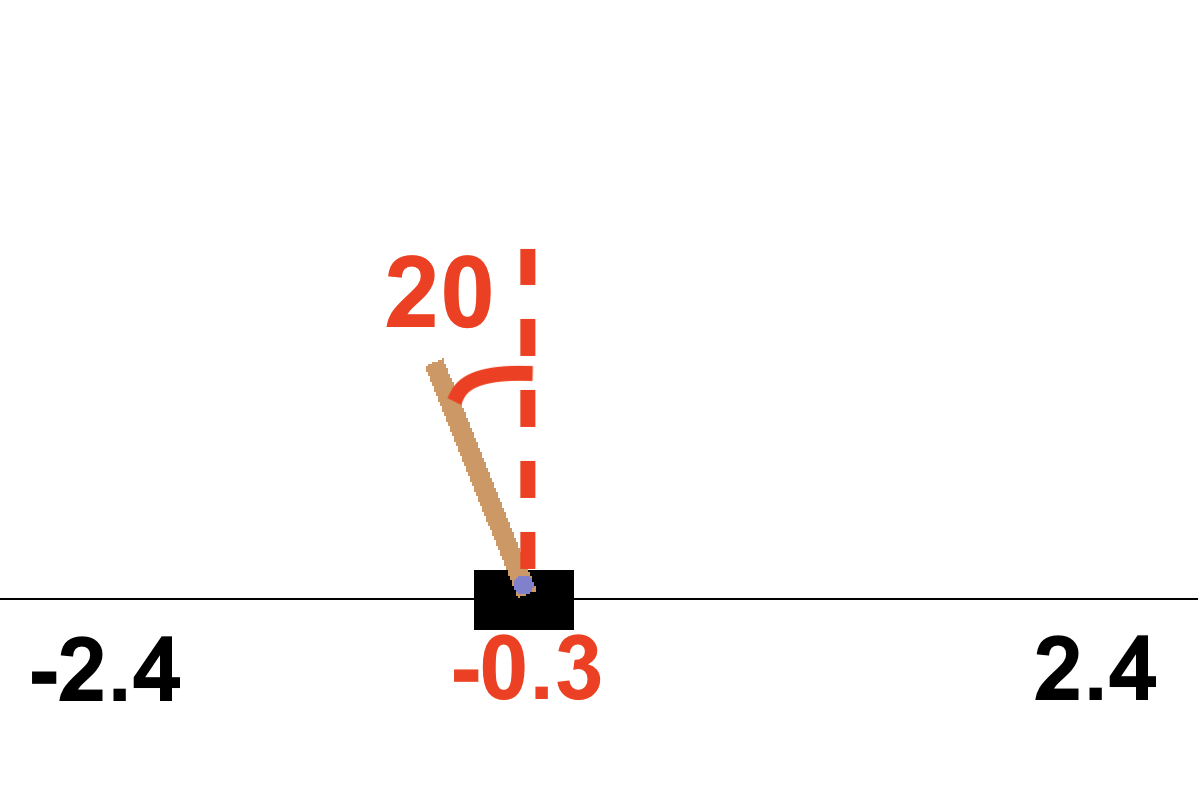
\includegraphics[width=\linewidth]{cartpole-v2.jpg}
	   \label{fig:cartpole-v1}
	\end{minipage}\hfill
}
\subfigure[]{
	\begin{minipage}[c][0.35\textwidth]{
	   0.45\textwidth}
	   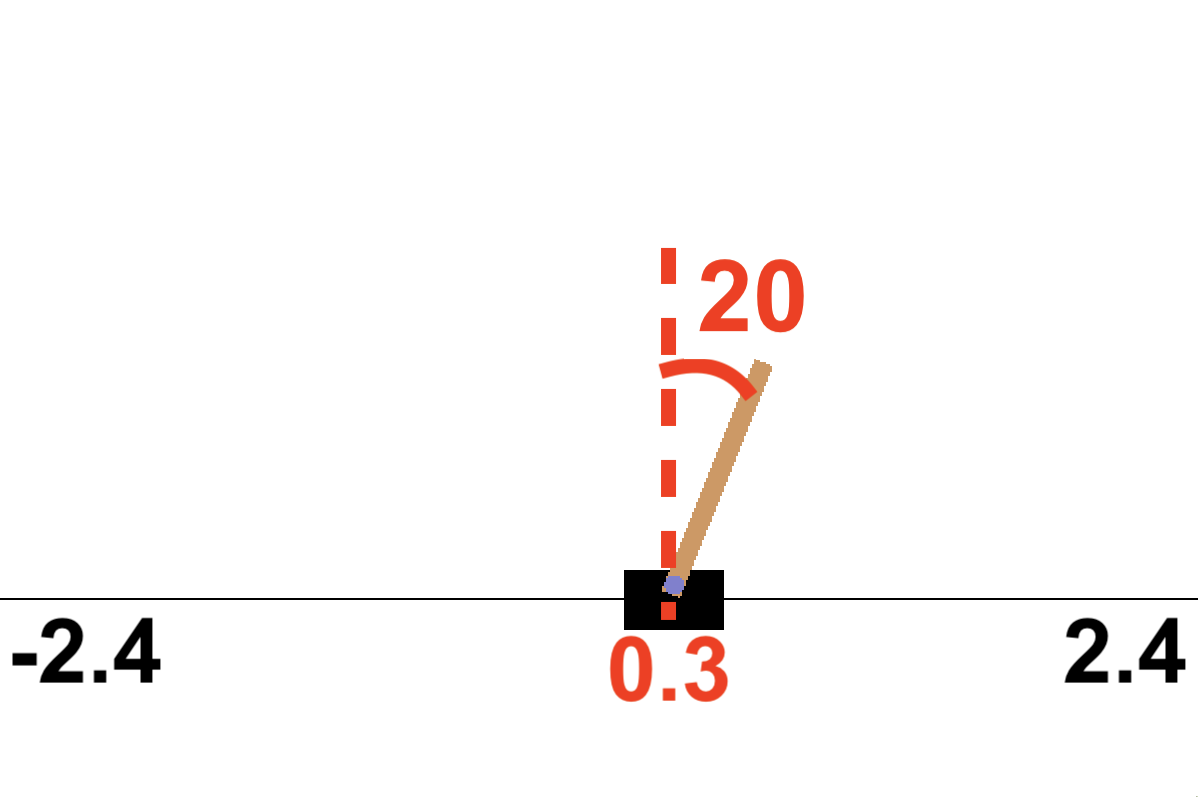
\includegraphics[width=\linewidth]{cartpole-v3.jpg}
	   \label{fig:cartpole-v2}
	\end{minipage}\hfill
}
%\vspace{-3mm} 
  \caption[The cartpole environment]{(a) The cartpole environment. (b) The cart is at -0.3 and pole angle is {-20}$^\circ$. (c) The cart is at 0.3 and pole angle is {20}$^\circ$.}    
\label{fig:cartpole}
%\vspace{-3mm}
\end{figure}
In grid world, it is hard to evaluate the performance that the agent may need to sacrifice for safety. Hence we implement the algorithm in OpenAI gym environments where performance can be quantified. In the cart-pole environment as shown in Fig.~\ref{fig:cartpole-v0}, the goal is to keep the pole on a cart from falling over as long as possible by moving the cart either to the left or to the right in each time step. The maximum step length is $t=200$. The position, velocity and angle of the cart and the pole are continuous values and observable, but the actual dynamics of the system are unknown.

We discretize the continuous observation space and formulate the environment as an MDP with 400 states and 2 actions. Through exploring the environment, the transition function is determined by the samples of experienced transitions. The feature vector in each state contains $30$ radial basis functions which depend on the squared Euclidean distances between current states and other $30$ states which are uniformly distributed in the state space. In addition, a maneuver is deemed {\it unsafe} if the pole angle is larger than 20$^\circ$ while the cart's horizontal position is more than $\pm 0.3$ as shown in Fig.~\ref{fig:cartpole-v1} and \ref{fig:cartpole-v2}. We formalize the safety requirement in PCTL as (\ref{eq:spec1}).
%\vspace{-2mm}
\begin{equation}
\begin{split}
\Phi ::= P_{\leq p^*}[true\ \until^{\leq t}\ &(angle\leq -20^\circ\wedge position\leq-0.3)\\
&\vee(angle\geq 20^\circ\wedge position\geq 0.3)]
\end{split}
\label{eq:spec1}
\end{equation}
%\vspace{-12mm}

\begin{table}[htb]
\begin{center}
\caption{In the cart-pole environment, {\it higher} average steps mean better performance. The safest policy is synthesized using PRISM-games.}
\begin{tabular}{|r|r|r|r|r|}
\hline
  &\small{\ \ MC Result} &\small{\ \ Avg. Steps}  &\small{\ \ Unsafe Rate} &\small{\ \ Num. of Iters}\\
\hline
AL &49.1\%& 165 &  19\% & 2\\
\hline
Safest Policy  & 0.0\% & 8 & 0.0\% & N.A.\\
\hline
$p^*=30\%$ & 17.2\%  & 121 & 13.0\% & 9\\
\hline
$p^*=25\%$ & 9.3\%  & 136 & 17.0\% & 13\\
\hline
$p^*=20\%$ & 17.2\% & 122 & 10.8\% & 8\\
\hline
$p^*=15\%$ & 7.3\% & 138 & 15.4\% & 21\\
\hline
$p^*=10\%$ & 7.2\% & 136 & 13.7\% & 21\\
\hline
$p^*=5\%$ & 0.04\% & 83 & 0.5\% & 50\\
\hline
\end{tabular}
\label{tab:cartpole1}
\end{center}
\end{table}
%\vspace{-10mm}

We consider only demonstrations for which the pole is held upright without violating any of the safety conditions for all 200 steps. The safest policy synthesized by PRISM-games is used as the initial safe policy. 
 We also compare the different policies learned by CEGAL for different safety threshold $p^*$s. 
In Table~\ref{tab:cartpole1}, the policies are compared in terms of model checking results (`MC Result') on the PCTL property in (\ref{eq:spec1}) using the constructed MDP, the average steps (`Avg. Steps') that a policy (executed in the OpenAI environment) can hold across $5000$ rounds (the higher the better), and averaged percentage times (`Unsafe Rate') that a policy (executed in the OpenAI environment) violates the $unsafe$ conditions across $5000$ rounds. The last column in the table shows the averaged number of iterations for these algorithms to converge (with $50$ as the maximum number of iterations). 
The policy in the first row is the result of using AL alone. 
Observe that from $p^* = 30\%$ to $10\%$, the performance of the learnt policy is similar. However, when the safety threshold becomes very low, e.g., $p^*=5\%$, the performance of the learnt policy drops significantly. 
Observe also that the safest policy has the lowest performance amongst all. 
It corresponds to simply letting the pole fall and thus does not risk moving the cart out of the range [-0.3, 0.3]. 
 We note that the discrepancy between the `MC result' and the `unsafe rate' is due to the MDP abstraction of the actual game environment. The safety guarantee of the algorithm is based on the former and the latter is used for validation purposes. The discordances between model checking results and unsafe rates are due to the inaccurate transition function. Despite the inconsistency, the policies learnt via CEGAL still show lower frequency of reaching unsafe states than that via AL.

\section{Mountain-Car from OpenAI Gym}
%\vspace{-5mm} 
\begin{figure}[h]
\centering
\subfigure[]{
	\hspace{0.1\linewidth}\begin{minipage}[c][0.35\textwidth]{
	   0.45\textwidth}
	   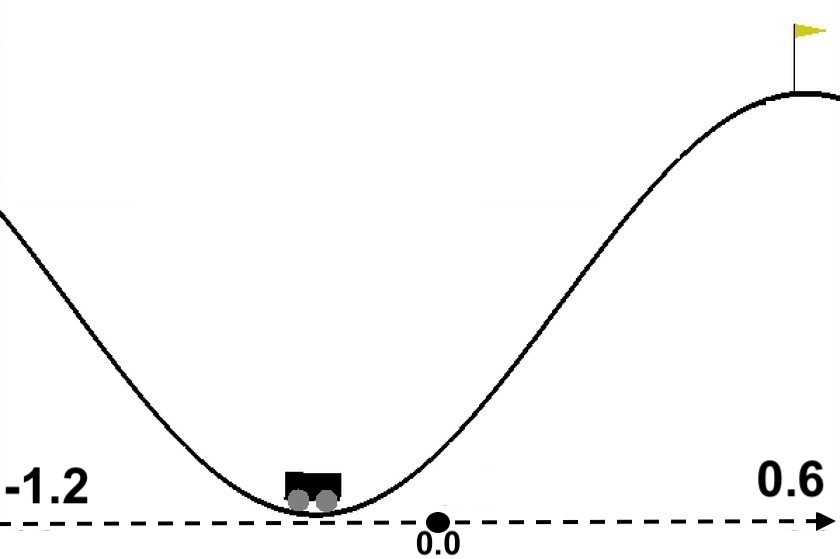
\includegraphics[width=1.2\linewidth]{mountaincar-v0.jpg}
	   \label{fig:mountaincar-v0}
	\end{minipage}\hspace{0.2\linewidth}
}
\subfigure[]{
	\begin{minipage}[c][0.35\textwidth]{
	   0.45\textwidth}
	   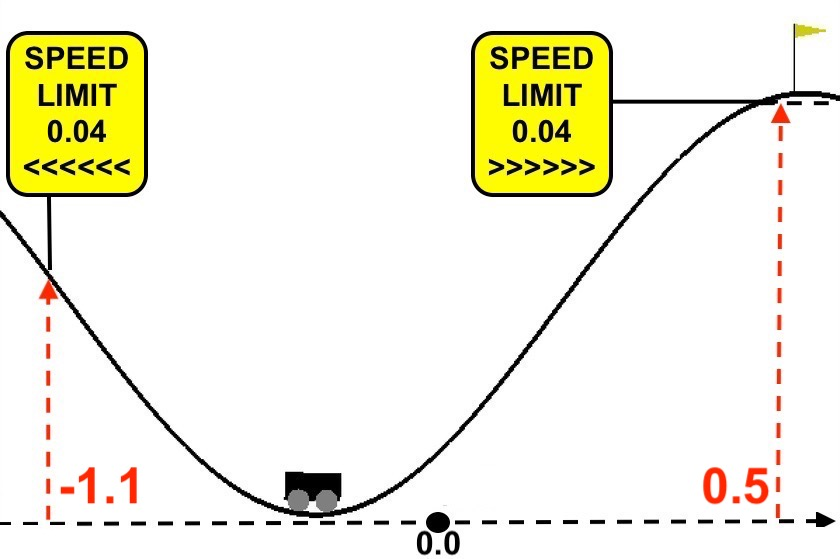
\includegraphics[width=1.2\linewidth]{mountaincar-v2.jpg}
	   \label{fig:mountaincar-v1}
	\end{minipage}\hspace{0.1\linewidth}
}
%\vspace{-3mm} 
\caption[The mountaincar environment]{(a) The original mountain-car environment. (b) The mountain-car environment with traffic rules: when the distance from the car to the left edge or the right edge is shorter than $0.1$, the speed of the car should be lower than $0.04$.}  
\label{fig:mountaincar}
\end{figure}

Our third experiment uses the mountain-car environment from OpenAI Gym. As shown in Fig. {\ref{fig:mountaincar-v0}}, a car starts from the bottom of the valley and tries to reach the mountaintop on the right as quickly as possible. In each time step the car can perform one of the three actions, accelerating to the left, coasting, and accelerating to the right. The agent fails if the step length reaches the maximum ($t=66$). The velocity and position of the car are continuous values and observable while the exact dynamics are unknown.

We discretize the continuous observation space and formulate the environment as an MDP with 320 states and 3 actions. Through exploring the environment, the transition function is determined by the samples of experienced transitions. The feature vector for each state contains 2 exponential functions and 18 radial basis functions which respectively depend on the squared Euclidean distances between the current state and other 18 states which are uniformly distributed in the state space. In this game setting, the car cannot reach the right mountaintop by simply accelerating to the right. It has to accumulate momentum first by moving back and forth in the valley. The safety rules we enforce are shown in Fig.~{\ref{fig:mountaincar-v1}. They correspond to speed limits when the car is close to the left mountaintop or to the right mountaintop (in case it is a cliff on the other side of the mountaintop). Similar to the previous experiments, we consider only expert demonstrations that successfully reach the right mountaintop without violating any of the safety conditions. 
The average step length of demonstrations is $40$. 
 We formalize the safety requirement in PCTL as (\ref{eq:spec2}). 

%\vspace{-5mm}
\begin{equation}
\begin{split}
\Phi ::= P_{\leq p^*}[true\ \until^{\leq t}\ &(speed\leq -0.04\wedge position\leq-1.1)\\
&\vee(speed\geq 0.04\wedge position\geq0.5)]
\end{split}
\label{eq:spec2}
\end{equation}
%\vspace{-2mm} 
\begin{table}[hbt]
\caption{In the mountain-car environment, {\it lower} average steps mean better performance. The safest policy is synthesized via PRISM-games.}
\begin{tabular}{|r|r|r|r|r|}
\hline 
\small{}  &\small{\ \ MC Result} &\small{\ \ Avg. Steps}  &\small{\ \ Unsafe Rate}&\small{\ \ Num. of Iters} \\ 
\hline \small
Policy Learnt via AL & 69.2\%& 54 & 100\% & 50\\
\hline
Safest Policy &  0.0\% &  $Fail$ & 0\% & 0\\
\hline
$p^*=60\%$&43.4\% & 57 & 33.2\% & 9\\
\hline
$p^*=50\%$ &46.9\%& 55 & 29.4\% & 23\\
\hline
$p^*=40\%$ &29.3\% & 61 & 0.6\% & 25\\
\hline
$p^*=30\%$ &18.9\% & 64 & 0.0\% & 17\\
\hline
$p^*=20\%$ &12.0\% & 66 & 3.5\% & 39\\
\hline
$p^*=10\%$ &7.6\% & $Fail$ & 0\%  & 40\\
\hline
\end{tabular}
\label{tab:mountaincar0}
%\vspace{-8mm}
\end{table}

 We compare the different policies using the same set of categories as in the cart-pole example. The numbers are averaged over 5000 rounds. The last column in the table shows the averaged number of iterations for these algorithms to converge (with $50$ as the maximum number of iterations).
As shown in the first row, the policy learnt via AL has the highest probability of going over the speed limits. We observe that this policy makes the car speed up all the way to the left mountaintop to maximize its potential energy. The safest policy corresponds to simply staying in the bottom of the valley. 
The policies learnt via CEGAL for the safety threshold $p^*$ ranges from $60\%$ to $50\%$ not only have lower probability of violating speed limits but also maintain comparable performance. However, when the safety threshold $p^*$ further decreases, the agent becomes more conservative and it takes more time for the car to finish the task. The discordances between model checking results and unsafe rates are due to the inaccurate transition function. Despite the inconsistency, the policies learnt via CEGAL still show obvious restraint in reaching unsafe states than that via AL.

\section{Discussion}
In the three experiments, we evaluate our algorithm in different aspects. From the gridworld experiment, we observe how safety specification influences the implicit search for reward function in our algorithm. When the safety threshold decreases, lower rewards will be assigned to the unsafe states so that the optimal policy with respect to the reward function will avoid reaching those states. From cart-pole and mountain-car experiments, we observe how our algorithm guarantees the safety of the final output policy while retaining the performance of the learnt policy in the mean time. In both experiments, by learning from human demonstrations and the counterexamples for violating the safety specification, the agent not only knows how to finish the tasks but also exhibits the awareness of safety.






